\documentclass[11pt,a4paper]{article}
\usepackage{fontspec}
\setmainfont{TeX Gyre Pagella}
\usepackage[a4paper,margin=2.2cm]{geometry}
\usepackage{graphicx,longtable,array,xcolor,float,caption}
\usepackage{xurl}
\usepackage[hidelinks]{hyperref}
\setlength{\parindent}{0pt}\setlength{\parskip}{0.55em}
\captionsetup{font=small,labelfont=bf}
\hypersetup{pdftitle={The AI Tapestry},pdfauthor={Tristan Hotham}}
\begin{document}
\begin{center}
{\Large\bfseries The AI Tapestry\par}\vspace{0.4em}
{\large An embroidered history of artificial intelligence, in the manner of the Bayeux Tapestry\par}\vspace{1.1em}
{\large Tristan Hotham\par}\vspace{0.3em}
{\small Independent researcher\\ ORCID: 0000-0003-4931-9349\\ DOI: \href{https://doi.org/10.5281/zenodo.23866754}{10.5281/zenodo.23866754}\par}\vspace{0.7em}
2026
\end{center}
\begin{quote}\small\begin{center}\textbf{Abstract}\end{center}
I present the history of artificial intelligence as a single scrolling strip in the visual language of the Bayeux Tapestry, the eleventh-century embroidery of the Norman conquest. 21 scenes run from Ada Lovelace's notes on the Analytical Engine (1843) to the AI agents of the mid-2020s, each with a caption in the dog Latin of the original, a plain English line, a short factual note and links to sources. The figures are drawn in code from a small kit of stitched shapes, so the cloth is generated from a list of scenes and can be extended as the history continues. The frame is chosen on purpose: the original is a long, partial account made for the winners, full of omens, feasts and fleets, and missing its end. The interactive version is at \url{https://maps.tristanhotham.com/ai-tapestry/}.
\end{quote}
\section*{1. Why a tapestry}
Histories of AI are usually told as timelines. A timeline gives every event the same weight and none of them a mood. The Bayeux Tapestry tells a story as a sequence of scenes in which people do things: they feast, point at a comet, build ships, swear oaths and fight, with Latin captions above and a running border of beasts and asides below. It is also openly partial. Treating the history of AI the same way makes room for the parts a timeline flattens: the boasts (the perceptron that would ``walk, talk, see, write''), the overconfidence (Dartmouth's ``2 month, 10 man study''), the winters, and the fact that the story has no end yet.
\section*{2. Method}
Every figure is drawn by code in SVG from a kit of parts in the manner of the original: oval heads with a cap of hair, short flared tunics with banded hems, coloured hose, stylised trees as dividers, and borders of paired beasts between diagonal bars. Fills imitate laid-and-couched work, rows of parallel wool held down by short stitches, and outlines imitate stem stitch, broken and slightly displaced so no line is ruler-straight. The palette follows the small range of natural dyes of the original: madder reds, weld yellows, woad blues, and greens from mixing them. Nothing is traced or copied from the tapestry itself.
Each scene is one entry in a list (\texttt{data/scenes.js}): a year, the Latin caption, its English, a note, sources, a width, the figures and objects to stitch, and optional marginal jokes for the borders. Adding a chapter is adding an entry. The notes are written to be accurate and fair rather than exhaustive, and every factual claim in them is linked to a source, mostly Wikipedia's articles and the primary papers and prize citations.
\section*{3. The scenes}
\begin{figure}[H]\centering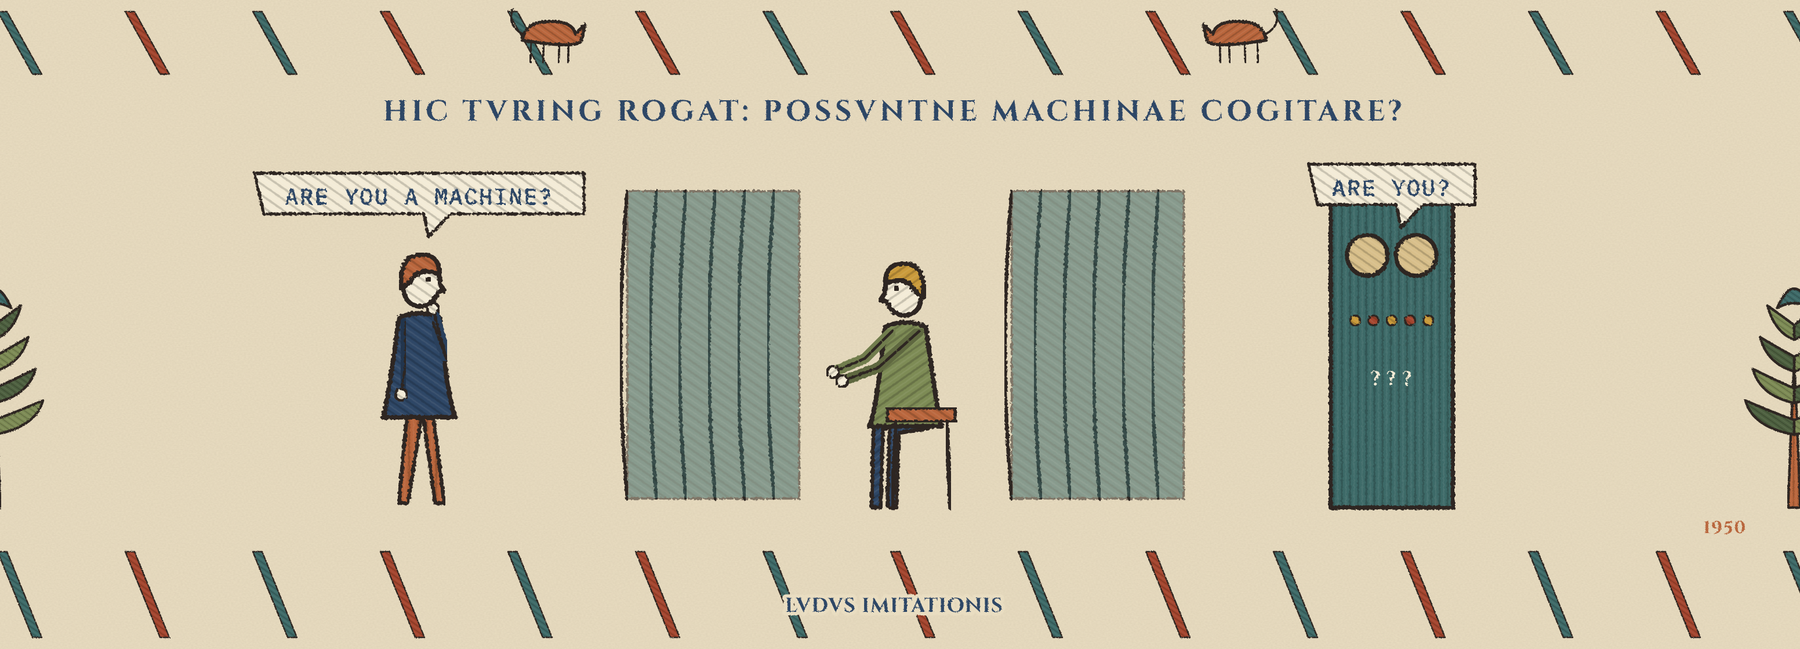
\includegraphics[width=\linewidth]{f_turing.png}\caption{1950: Turing's imitation game, played through a curtain.}\end{figure}
\begin{figure}[H]\centering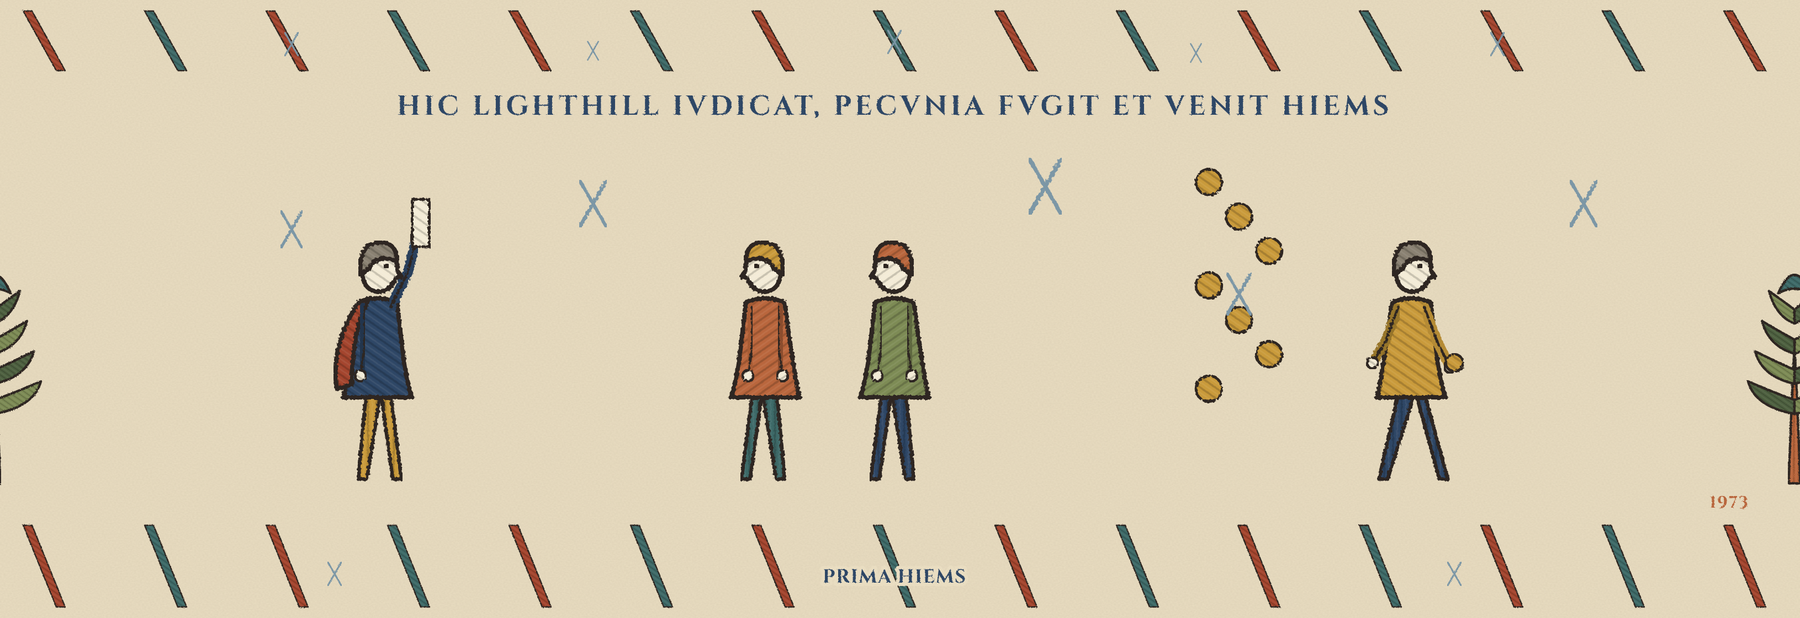
\includegraphics[width=\linewidth]{f_winter.png}\caption{1973: the Lighthill report and the first AI winter.}\end{figure}
\begin{figure}[H]\centering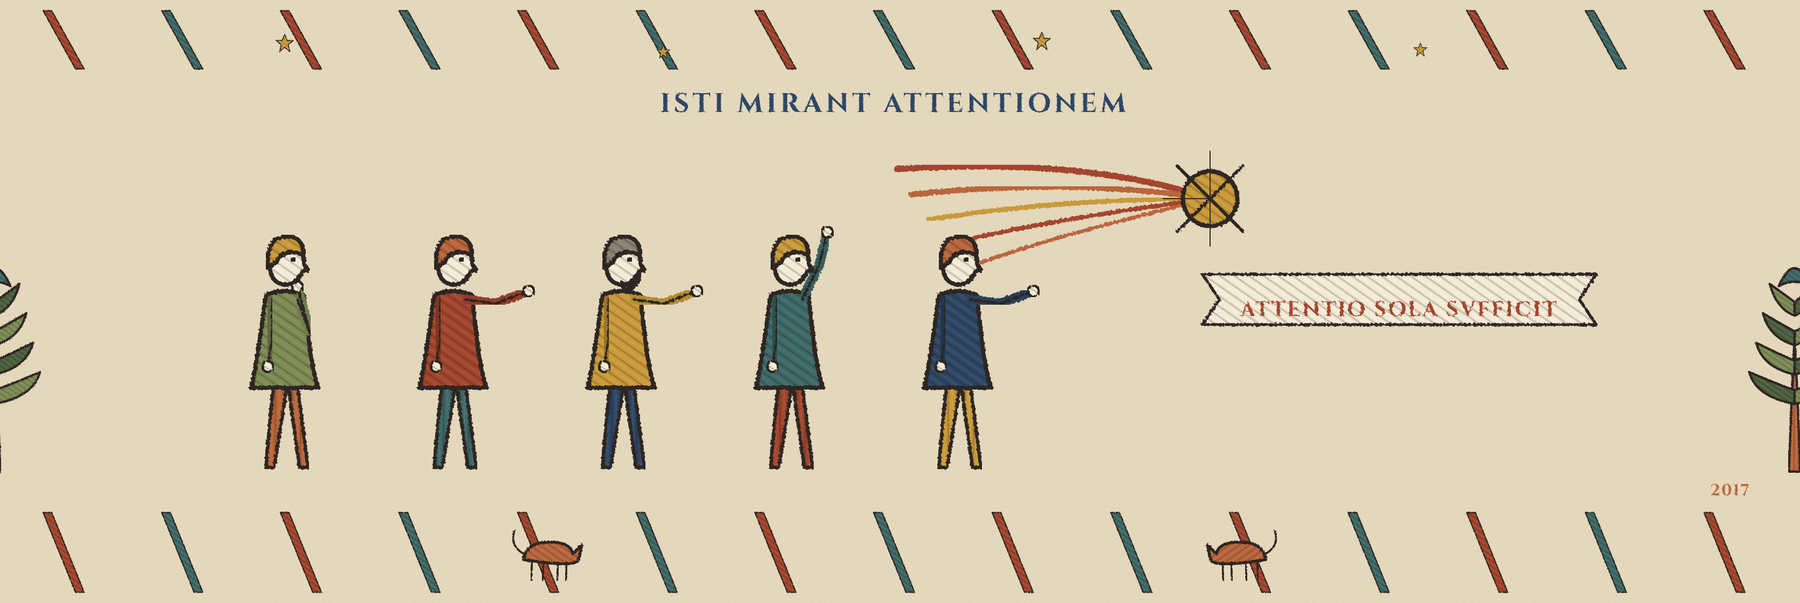
\includegraphics[width=\linewidth]{f_transformer.png}\caption{2017: ``ISTI MIRANT ATTENTIONEM'', after the comet scene of the original.}\end{figure}
\begin{figure}[H]\centering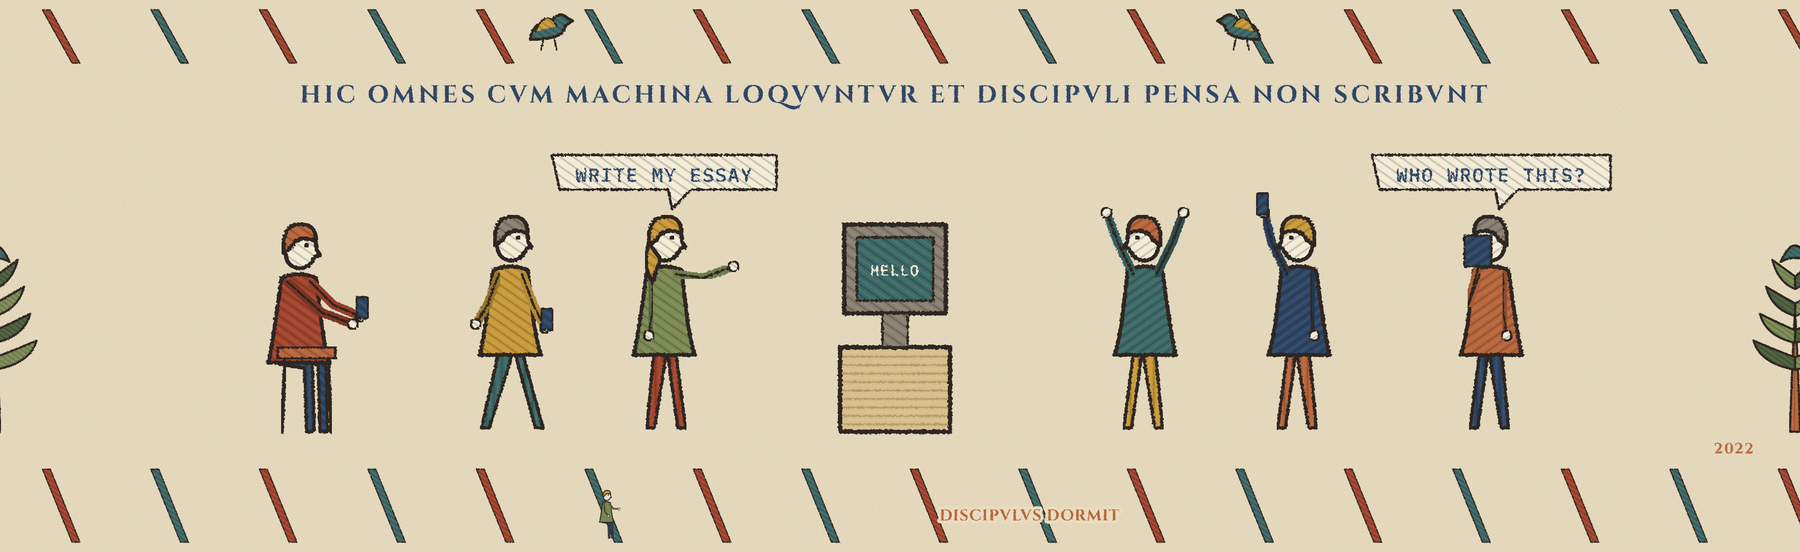
\includegraphics[width=\linewidth]{f_chatgpt.png}\caption{2022: everyone talks with the machine.}\end{figure}
{\small\begin{longtable}{>{\raggedright\arraybackslash}p{1.4cm}>{\raggedright\arraybackslash}p{14.4cm}}
\textbf{1843} & \textsc{hic ada notas scribit et machinam cantare somniat}\newline\emph{Here Ada writes her notes, and dreams that the engine might make music.}\newline Ada Lovelace translated an Italian paper on Charles Babbage's Analytical Engine and added notes three times its length. Note G sets out step by step how the engine could compute Bernoulli numbers, often called the first published computer program, and she guessed it might one day compose music. She also wrote that it could only do what we know how to order it to do: the first objection to machine intelligence, and one Turing answered by name. The engine itself was never finished.\newline{\footnotesize Sources: \href{https://en.wikipedia.org/wiki/Ada_Lovelace}{Ada Lovelace (Wikipedia)}; \href{https://en.wikipedia.org/wiki/Analytical_Engine}{Analytical Engine (Wikipedia)}}\\[4pt]
\textbf{1950} & \textsc{hic tvring rogat: possvntne machinae cogitare?}\newline\emph{Here Turing asks: can machines think?}\newline In ``Computing Machinery and Intelligence'' Alan Turing swapped an unanswerable question for a game: if a judge, talking by typed messages, cannot tell a machine from a person, what grounds are left for saying it does not think? He predicted that by about the year 2000 machines would fool an average judge for five minutes 30 per cent of the time, and he answered nine objections in advance, including ``Lady Lovelace's''.\newline{\footnotesize Sources: \href{https://en.wikipedia.org/wiki/Computing_Machinery_and_Intelligence}{Computing Machinery and Intelligence (Wikipedia)}; \href{https://en.wikipedia.org/wiki/Turing_test}{Turing test (Wikipedia)}}\\[4pt]
\textbf{1956} & \textsc{hic docti dartmvthiae convenivnt et vnam aestatem svfficere pvtant}\newline\emph{Here the learned meet at Dartmouth and reckon one summer will be enough.}\newline The proposal for the Dartmouth Summer Research Project, which coined the name ``artificial intelligence'', asked for ``a 2 month, 10 man study'' and hoped that ``a significant advance can be made'' on language, abstraction and self-improvement ``if a carefully selected group of scientists work on it together for a summer''. It was organised by John McCarthy, Marvin Minsky, Nathaniel Rochester and Claude Shannon. The summer has lasted rather longer.\newline{\footnotesize Sources: \href{https://en.wikipedia.org/wiki/Dartmouth_workshop}{Dartmouth workshop (Wikipedia)}; \href{http://jmc.stanford.edu/articles/dartmouth/dartmouth.pdf}{The 1955 proposal (Stanford, J. McCarthy)}}\\[4pt]
\textbf{1958} & \textsc{hic rosenblatt perceptronem facit et praecones eam ambvlatvram clamant}\newline\emph{Here Rosenblatt makes the perceptron, and the heralds cry that it will walk.}\newline Frank Rosenblatt's perceptron learned to sort simple pictures by adjusting the weights on its connections, the ancestor of every neural network since. The New York Times reported that the Navy expected it to be the ``embryo of an electronic computer'' that would ``walk, talk, see, write, reproduce itself and be conscious of its existence''. The Mark I Perceptron was a cabinet of wires and motor-driven dials with a 20 by 20 grid of light cells for an eye.\newline{\footnotesize Sources: \href{https://en.wikipedia.org/wiki/Perceptron}{Perceptron (Wikipedia)}; \href{https://en.wikipedia.org/wiki/Frank_Rosenblatt}{Frank Rosenblatt (Wikipedia)}}\\[4pt]
\textbf{1966} & \textsc{hic eliza avscvltat et homines ei secreta narrant}\newline\emph{Here ELIZA listens, and people tell it their secrets.}\newline Joseph Weizenbaum's ELIZA ran a script called DOCTOR that played a psychotherapist by turning what you typed back into a question. Weizenbaum was dismayed at how quickly people confided in it; he wrote that his secretary, who had watched him build it, asked him to leave the room so she could talk to it in private. He spent much of his later career warning against handing human judgement to machines.\newline{\footnotesize Sources: \href{https://en.wikipedia.org/wiki/ELIZA}{ELIZA (Wikipedia)}; \href{https://en.wikipedia.org/wiki/Joseph_Weizenbaum}{Joseph Weizenbaum (Wikipedia)}}\\[4pt]
\textbf{1973} & \textsc{hic lighthill ivdicat, pecvnia fvgit et venit hiems}\newline\emph{Here Lighthill gives his verdict, the money flees and winter comes.}\newline After Minsky and Papert showed in 1969 what a single-layer perceptron could not learn, and the grand promises of the 1960s went unmet, funding dried up. In Britain, Sir James Lighthill's 1973 report to the Science Research Council found that no part of the field had made the major impact once promised, and most British AI research lost its funding; in the United States, the military agency DARPA cut back. The lean years became known as the first AI winter.\newline{\footnotesize Sources: \href{https://en.wikipedia.org/wiki/Lighthill_report}{Lighthill report (Wikipedia)}; \href{https://en.wikipedia.org/wiki/AI_winter}{AI winter (Wikipedia)}}\\[4pt]
\textbf{1980} & \textsc{hic mercatores regvlas vendvnt: si hoc, tvnc illvd}\newline\emph{Here the merchants sell rules: if this, then that.}\newline The 1980s boom ran on expert systems: thousands of hand-written if-then rules distilled from specialists. XCON, built for Digital Equipment Corporation, configured computer orders and was said to save the firm tens of millions of dollars a year. Japan launched its Fifth Generation Computer project, specialised LISP machines were sold to run it all, and then the market for them collapsed in 1987, bringing a second winter: the rules were brittle, expensive to keep up and could not learn.\newline{\footnotesize Sources: \href{https://en.wikipedia.org/wiki/Expert_system}{Expert system (Wikipedia)}; \href{https://en.wikipedia.org/wiki/Xcon}{Xcon (Wikipedia)}; \href{https://en.wikipedia.org/wiki/Lisp_machine}{Lisp machine (Wikipedia)}}\\[4pt]
\textbf{1986} & \textsc{hic errores retro propagantvr et retia discvnt}\newline\emph{Here the errors are passed back and the networks learn.}\newline Rumelhart, Hinton and Williams showed in Nature how networks with hidden layers could learn by passing their errors backwards through the connections, nudging every weight a little: backpropagation. The idea had earlier roots, but this paper made it work and spread it. It is still how almost every neural network is trained, and it answered the limits Minsky and Papert had found in the single-layer perceptron.\newline{\footnotesize Sources: \href{https://en.wikipedia.org/wiki/Backpropagation}{Backpropagation (Wikipedia)}; \href{https://doi.org/10.1038/323533a0}{Learning representations by back-propagating errors (Nature, 1986)}}\\[4pt]
\textbf{1997} & \textsc{hic caervlevs profvndvs kasparovvm vincit}\newline\emph{Here Deep Blue defeats Kasparov.}\newline IBM's Deep Blue beat the world chess champion Garry Kasparov over six games in New York, the first time a computer had won a match against a reigning champion under tournament conditions. It won by brute force and expert-tuned evaluation, searching up to about 200 million positions a second, not by learning. Kasparov suspected human help and asked for a rematch; IBM retired the machine.\newline{\footnotesize Sources: \href{https://en.wikipedia.org/wiki/Deep_Blue_versus_Garry_Kasparov}{Deep Blue versus Garry Kasparov (Wikipedia)}}\\[4pt]
\textbf{2011} & \textsc{hic watson in lvdo interrogationvm vincit}\newline\emph{Here Watson wins at Jeopardy!}\newline IBM's Watson beat the two most successful Jeopardy! champions, Ken Jennings and Brad Rutter, on television, answering clues written in puns and wordplay. Jennings added to his final answer: ``I for one welcome our new computer overlords.'' Watson was later sold for medicine, with mixed results.\newline{\footnotesize Sources: \href{https://en.wikipedia.org/wiki/IBM_Watson}{Watson (computer) (Wikipedia)}}\\[4pt]
\textbf{2012} & \textsc{hic machinae feles vident et fornaces graphicae ardent}\newline\emph{Here the machines see cats, and the graphics furnaces burn.}\newline AlexNet, by Alex Krizhevsky, Ilya Sutskever and Geoffrey Hinton, won the ImageNet image-recognition contest by a wide margin, a deep neural network trained on two gaming graphics cards. The same year a Google network, shown frames from YouTube, learned on its own to respond to cats. Deep learning took over the field, and graphics chips became the furnaces of a new industry.\newline{\footnotesize Sources: \href{https://en.wikipedia.org/wiki/AlexNet}{AlexNet (Wikipedia)}; \href{https://en.wikipedia.org/wiki/ImageNet}{ImageNet (Wikipedia)}}\\[4pt]
\textbf{2016} & \textsc{hic alphago motvm xxxvii facit et omnes mirantvr}\newline\emph{Here AlphaGo plays move 37 and everyone marvels.}\newline DeepMind's AlphaGo beat Lee Sedol, one of the strongest Go players of the age, four games to one in Seoul. In game two its 37th move, a shoulder hit on the fifth line, looked like a mistake to every professional watching; commentators later called it beautiful. In game four Lee found a move of his own, his 78th, that AlphaGo had not foreseen, and won: the only game a human took from it.\newline{\footnotesize Sources: \href{https://en.wikipedia.org/wiki/AlphaGo_versus_Lee_Sedol}{AlphaGo versus Lee Sedol (Wikipedia)}}\\[4pt]
\textbf{2017} & \textsc{isti mirant attentionem}\newline\emph{These people marvel at the attention.}\newline A paper by eight Google researchers, ``Attention Is All You Need'', introduced the transformer, which weighs every word against every other word at once instead of reading in order. It trains well on huge numbers of chips in parallel, and it is the T in GPT. The caption borrows from the most famous scene in the original, where people stare and point at a comet: ISTI MIRANT STELLA, these people marvel at the star.\newline{\footnotesize Sources: \href{https://en.wikipedia.org/wiki/Attention_Is_All_You_Need}{Attention Is All You Need (Wikipedia)}; \href{https://en.wikipedia.org/wiki/Transformer_(deep_learning_architecture)}{Transformer (Wikipedia)}}\\[4pt]
\textbf{2019} & \textsc{hic fabri dicvnt: nimis pericvlosvm est, et clavdvnt}\newline\emph{Here the makers say it is too dangerous, and lock it away.}\newline OpenAI announced GPT-2, a language model that wrote startlingly fluent paragraphs, and at first held back the full version for fear of misuse, releasing it in stages over nine months. Many researchers thought the caution overdone; others saw it as the first time a lab had tried a staged release. A year later GPT-3, more than a hundred times larger, showed that simply making models bigger kept making them better.\newline{\footnotesize Sources: \href{https://en.wikipedia.org/wiki/GPT-2}{GPT-2 (Wikipedia)}; \href{https://en.wikipedia.org/wiki/GPT-3}{GPT-3 (Wikipedia)}}\\[4pt]
\textbf{2020} & \textsc{hic proteina plicantvr et qvaestio qvinqvaginta annorvm solvitvr}\newline\emph{Here the proteins fold, and a fifty-year question is answered.}\newline DeepMind's AlphaFold 2 predicted the 3D shapes of proteins from their sequence of amino acids about as accurately as laboratory methods, in the CASP14 assessment. Working out how a chain of amino acids folds had been a central puzzle of biology for half a century. In 2022 the team released predicted structures for some 200 million proteins, nearly every one known to science.\newline{\footnotesize Sources: \href{https://en.wikipedia.org/wiki/AlphaFold}{AlphaFold (Wikipedia)}}\\[4pt]
\textbf{2022} & \textsc{hic omnes cvm machina loqvvntvr et discipvli pensa non scribvnt}\newline\emph{Here everyone talks with the machine, and the students stop writing their homework.}\newline OpenAI released ChatGPT as a ``research preview''. It reached a million users in five days and an estimated 100 million in two months, then the fastest-growing consumer app on record. Teachers rethought essays, lawyers were caught citing cases it had invented, and rival chatbots followed within months, among them Google's Bard and Anthropic's Claude, the model that helped stitch this tapestry.\newline{\footnotesize Sources: \href{https://en.wikipedia.org/wiki/ChatGPT}{ChatGPT (Wikipedia)}}\\[4pt]
\textbf{2023} & \textsc{hic principes apvd bletchley convivant et de pericvlis dispvtant}\newline\emph{Here the great and good dine at Bletchley and debate the dangers.}\newline Representatives of 28 countries and the EU met at Bletchley Park, where Turing had broken codes in the war, for the first AI Safety Summit, and signed a declaration that frontier AI could cause ``serious, even catastrophic, harm''. The scene borrows the original's feast, where a bishop blesses the food before the battle. Some critics found the focus on far-off risks a distraction from present harms; follow-up summits were held in Seoul and Paris.\newline{\footnotesize Sources: \href{https://en.wikipedia.org/wiki/AI_Safety_Summit}{AI Safety Summit (Wikipedia)}; \href{https://www.gov.uk/government/publications/ai-safety-summit-2023-the-bletchley-declaration}{Bletchley Declaration (GOV.UK)}}\\[4pt]
\textbf{2024} & \textsc{hic praemia nobeliana retivm magistris dantvr}\newline\emph{Here the Nobel prizes go to the masters of the networks.}\newline The Nobel Prize in Physics went to John Hopfield and Geoffrey Hinton for the foundations of machine learning with artificial neural networks; the Chemistry prize went to Demis Hassabis and John Jumper for AlphaFold, shared with David Baker for designing new proteins. Hinton, who had left Google the year before so he could speak freely about the risks, used his acceptance to warn about them.\newline{\footnotesize Sources: \href{https://www.nobelprize.org/prizes/physics/2024/summary/}{2024 Nobel Prize in Physics (NobelPrize.org)}; \href{https://www.nobelprize.org/prizes/chemistry/2024/summary/}{2024 Nobel Prize in Chemistry (NobelPrize.org)}}\\[4pt]
\textbf{2025} & \textsc{hic balaena ab oriente venit et avrvm mercatorvm cadit}\newline\emph{Here a whale comes from the east, and the merchants' gold falls.}\newline The Chinese lab DeepSeek, whose logo is a whale, released R1, an openly published reasoning model that rivalled the best American systems at a reported fraction of the training cost. The next trading day the chipmaker Nvidia lost about \$590 billion of market value, the largest one-day fall in US stock-market history, before recovering. Reasoning models, which work through problems step by step before answering, became the new frontier.\newline{\footnotesize Sources: \href{https://en.wikipedia.org/wiki/DeepSeek}{DeepSeek (Wikipedia)}; \href{https://en.wikipedia.org/wiki/Nvidia}{Nvidia (Wikipedia)}}\\[4pt]
\textbf{2025} & \textsc{hic machinae per se laborant et homines eas specvlantvr}\newline\emph{Here the machines work by themselves, and people watch over them.}\newline By the mid-2020s AI systems were being given tools and set to work on long tasks: writing and running code, browsing, filling in forms, carrying out research for hours with little supervision. The questions moved from what the models know to what they should be allowed to do, and who checks their work. This scene is where the history meets the present, and it will need re-stitching.\newline{\footnotesize Sources: \href{https://en.wikipedia.org/wiki/Intelligent_agent}{Intelligent agent (Wikipedia)}; \href{https://en.wikipedia.org/wiki/AI_agent}{AI agent (Wikipedia)}}\\[4pt]
\textbf{MMXXVI} & \textsc{hic tela nondvm finita est}\newline\emph{Here the cloth is not yet finished.}\newline The real tapestry is missing its end: the last scenes were lost, and the stitched edge now stops part-way through the story. This one is unfinished on purpose. New scenes will be added as the history happens. If you think something important is missing, or told unfairly, say so.\newline{\footnotesize Sources: \href{https://en.wikipedia.org/wiki/Bayeux_Tapestry}{Bayeux Tapestry (Wikipedia)}}\\[4pt]
\end{longtable}}
\section*{4. Limits}
A tapestry chooses. These scenes favour landmark results and public moments over the slow accumulation of methods, data and hardware that made them possible, and they lean towards work in Britain and the United States. Many people who mattered are absent. The Latin is deliberately the loose Latin of the original, and the jokes are mine. The scene list is open, and the cloth is meant to be added to and corrected.
\section*{Data and code}
Scenes, drawing code, figures and this paper: \url{https://github.com/Tristan-Hotham/ai-tapestry} and DOI \href{https://doi.org/10.5281/zenodo.23866754}{10.5281/zenodo.23866754}. Code MIT; text and figures CC BY 4.0. The author used an AI system to help draft code and text, and checked every factual claim against the sources given.
\end{document}
